\chapter{Progress towards studies of quantum magnetism}
\label{ch:chap6}

A straightforward extension of the work presneted in this thesis would be to control interparticle spacing via an optical lattice. For these and additional experiments using quantum degenerate fermionic strontium we purchased and installed an optical lattice system. Our lattice is implemented using a Coherent Verdi V-18 which is shapped and propagated to our science chamber in free space. \hl{Fig} shows the optical path for each arm of our cubic lattice. 

Unfortunately, complications due to heating when loading the lattice has limited our success in this optical trap. I want to go over what we have been able to do so far with the lattice.

How did we characterize?
	Kaptiza-dirac extension
	
What convinced us we were having problems?

What are some ideas we could do in the lattice?
	Zeno
	faster cooling via stimulated raman potentailly? (can I model this somehow?)
	repulzively bound molecules?
	use interaction control in lattice with the zeno thing
	

\section{Spin manipulation of $^{87}$Sr}
\label{sec:spin_pol}

Here is where I need to introduce and characterize the \hl{LCR}

Averaging images together (how to use this code specifcally)

don't forget to talk about optimizing the polarization of the fixed waveplate

Fig. \hl{something} shows the variation of the retardance angle for 689\,nm light.

For reference, Fig. \ref{fig:mF87} reproduces the Clebsch-Gordan coefficient diagrams originally created by Pascal.
From this diagram we can easily see how optical pumping works.
Let us consider an atom starting in the $m_F=-9/2$ ground state and being exposed to $sigma+$ photons acting on the $F=9/2\,\rightarrow\,F=11/2$ hyperfine transition.
Absorbing a photon promotes the atom to the $F=11/2, m_F=-7/2$ state.
From here we can consult Fig. \ref{fig:mF87} to find the dominate decay path to be to the $F=9/2, m_F=-5/2$ state due to the Clebsch-Gordan coefficients.

Now we have a couple of options, by taking advanatage of the CG coefficents we see that we will probabilitically promote population towards a polarized state.
In the absecene of a bias field the magnetic sub-levels are degenerate so this oculd be an efficeint process.
In practice we find this to heat the atom population significantly.
Therefore, in a bias field, we split out the levels by approx. 200\,kHz to and address each sub-level transition individually.
This allows us to minimize the number of photon scattering events which we hypothesize to be the cause of the observed heating.

can individually address the separate hyperfine sub-level transitions and sequentially pump population towards one a polarized state 
	\begin{figure}
		\centerline{
		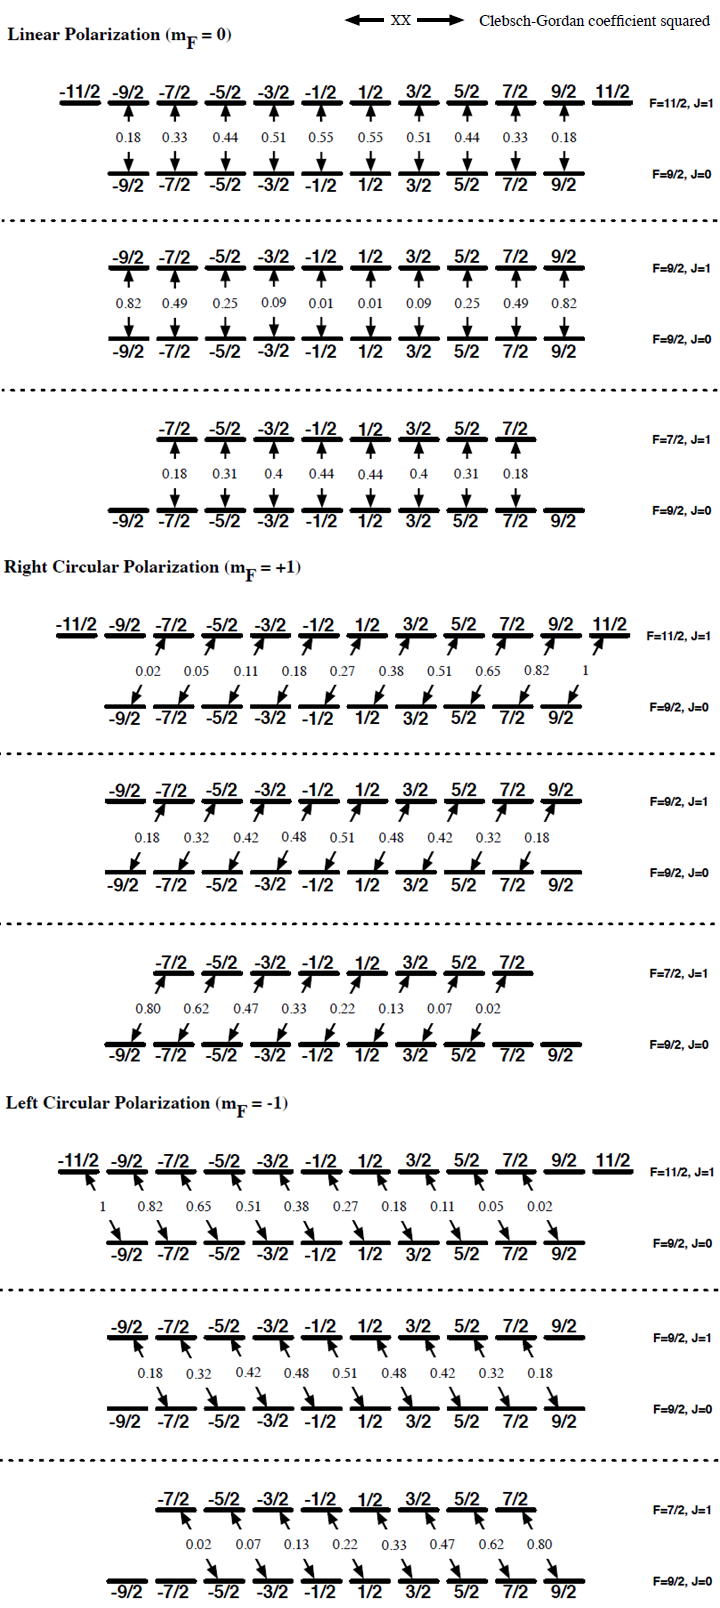
\includegraphics[height=\textheight]{87_CG_coeffs.png}}
		\caption{$^{87}$Sr $^1S_0 \, \rightarrow \, ^3P_1$ hyperfine structure}
		\label{fig:mF87}
	\end{figure} 
	
Be sure to define convention for what we determined was plus and minus

\section{Search for narrowline PA molecules using various spin mixtures}
\label{sec:87PAS}

"Lorem ipsum dolor sit amet, consectetur adipiscing elit, sed do eiusmod tempor incididunt ut labore et dolore magna aliqua. Ut enim ad minim veniam, quis nostrud exercitation ullamco laboris nisi ut aliquip ex ea commodo consequat. Duis aute irure dolor in reprehenderit in voluptate velit esse cillum dolore eu fugiat nulla pariatur. Excepteur sint occaecat cupidatat non proident, sunt in culpa qui officia deserunt mollit anim id est laborum."